\section*{System Track Benchmark Framework}
% Target word count between 750 and 1000.

While the algorithm track aims to benchmark solutions in a system-independent manner via complexity analysis, the NeuroBench system track aims to evaluate deployed execution time, throughput, and efficiency of systems comprised of an algorithm deployed and tailored to a hardware platform. \secondrev{Previous benchmark studies have examined neuromorphic systems under various applications, including keyword spotting~\cite{blouw2019, bos2024micropowerspokenkeywordspotting}, audio and video processing~\cite{shrestha24efficient}, and combinatorial optimization~\cite{chen2024onoffneuromorphicisingmachines, pierro2024solvingquboloihi2}. While these studies have demonstrated neuromorphic system advantages, the benchmark tasks have been unaligned. In order for the hallmarks of neuromorphic hardware to be aptly judged against conventional systems and foster the expansion of neuromorphic solutions, transparent and objective comparisons must be made on standard tasks between sufficiently mature neuromorphic systems head-to-head, as well as against conventional systems.}

    \begin{figure}[ht]
            \centering
            
\includegraphics[width=.85\textwidth]{figures/system_types.png}
            \caption{Types of neuromorphic systems at various integration scales.}
        \label{fig:system_types}
    \end{figure}

A key challenge for benchmarking neuromorphic hardware is that systems are implemented and deployed at vastly different scales to serve diverse applications, from cloud services (e.g., multi-chip platforms like Loihi~\cite{Davies18loihi} and SpiNNaker~\cite{mayr2019spinnaker}) to embedded sensing intelligence (e.g., Speck~\cite{synsensespeck} and SNP~\cite{InnateraSNP, Levy2021}). This range is visualized in Figure~\ref{fig:system_types}. \secondrev{Existing benchmarks for conventional systems have individual focuses across high-performance~\cite{top500}, datacenter-level computing~\cite{Reddi2020}, and embedded processing~\cite{banbury2021mlperf}. 
Thus, rather than pursuing a one-size-fits-all suite of tasks, the goal of the NeuroBench system track is to develop benchmarks at various scales and use cases, under multiple application areas in which both conventional and neuromorphic platforms may compete. The selected v1.0 NeuroBench system track benchmarks represent key commercial application areas for existing systems, and they differ from the tasks in the algorithm track, which are more research-oriented. As benchmark results continue to identify properties of highly effective algorithms and systems, the two tracks will converge to the same selction of tasks that are seen as the most impactful for future progress in the field.}

\secondrev{In this section, we present the system track guidelines outlining metrics and tasks, representing collective design between multiple owners and vendors of neuromorphic hardware. Baseline benchmark results for neuromorphic and conventional systems are reported, and further official results will be collected and announced at a regular cadence, akin to the MLPerf suite~\cite{mlperf_policies}. As with all other facets of the NeuroBench framework, the system track guidelines will continue to be adapted and extended iteratively as benchmark results are produced and shared. Up-to-date information on the latest benchmarks and official results can be found on the NeuroBench website (\url{https://neurobench.ai/}).}

% As the system track benchmark tooling is currently under development, insight from the algorithm track's early results will be exploited towards a future release of the detailed harness documentation, benchmark procedure, and baselines for the system track by the end of 2024.

    \subsection*{System Track Metrics}
    \secondrev{In order to be representative of the properties of a deployed system, the system benchmarks, like the algorithm benchmarks, are assessed at the task level for the overall system, as opposed to operation- or kernel-level assessment of individual components. Task-level benchmarks enable straightforward comparison between systems of any type with regard to their abilities to solve problems, and the overall system-level measurement describes the realistic capability and efficiency of a whole solution.}

    \secondrev{Each individual system benchmark uses task-specific metrics aligned with \textit{correctness}, \textit{timing}, and \textit{efficiency} to measure the system under test (SUT). The following general considerations are applied to each category:}
    % % The following performance metrics describe what is considered a system-level evaluation. 
    % \sout{For ease of comparison and benchmark result analysis, key features of the NeuroBench system track are consistent with features from the widely-adopted machine learning  system benchmark MLPerf Inference~\cite{Reddi2020}.}

    % \TODO{Remove details about Task Scenarios, since it doesn't appear that the system benchmarks are consistent enough with the different scenarios. Make sure that the content serves the results report from Xylo.}

    % \paragraph{Task Scenarios.} Where applicable, the NeuroBench system track will utilize benchmark task scenarios from MLPerf. MLPerf describes task scenarios under which system benchmarks are presented to the system under test (SUT). For large-scale batched processing, MLPerf defines the \textbf{Offline} and \textbf{Server} scenarios, which are latency-unconstrained and latency-constrained, respectively, with performance measured in terms of prediction throughput. For batch-size-1 processing, MLPerf defines \textbf{Single-stream} scenarios, for which performance is measured in terms of prediction latency.

    % However, the MLPerf task scenarios all consider data as discrete samples, and therefore do not fit with some key neuromorphic system applications. The NeuroBench system track thus defines two additional task scenarios: \textbf{Real-time} and \textbf{Optimization}. \textit{Real-time} uses continuous data streams (e.g., from an event camera), which must be processed online by the SUT, in contrast with the \textit{Single-stream} scenario, where samples are sent only once the SUT has completed processing. Optimization applications use heuristic methods for otherwise intractable problems, and thus do not have notions of sample throughput or sample latency. The \textit{Optimization} scenario benchmarks will report latency for the SUT to reach multiple correctness thresholds, as many approaches find sucessively improved solutions over time.
    

    % For each task and scenario, the following metric categories are reported:
    \begin{itemize}
        \item \textbf{Correctness} -- \secondrev{In other system benchmarks, such as the closed category of the MLPerf Inference framework~\cite{Reddi2020}, the same trained model is used to benchmark all SUTs, and a correctness threshold is imposed to ensure optimizations such as lower precision do not disrupt task performance.}
        
        Due to the tight coupling between an algorithm and its system implementation in many existing neuromorphic hardware solutions, the particular model used to solve a NeuroBench system track benchmark task is unconstrained. Therefore, correctness must be measured to verify the validity of the solution. No correctness thresholds are imposed on submissions, but the benchmark leaderboard will impose tiers of solution correctness on submissions to evaluate accuracy-efficiency trade-offs of system approaches.
        
        \item \textbf{Timing} -- \secondrev{Depending on the task, timing performance can include measurements of sample throughput or execution time. Individually, the former entails an offline, batched inference benchmark, while the latter aligns with a streaming benchmark, in which one inference does not start until the previous one ends. Together, both throughput and execution time should be reported for tasks in which the SUT runs multiple inferences at any given time, each representing a request which must be responded to within a constrained window. The MLPerf Inference framework has defined widely-adopted general task scenarios corresponding to each of these categories (offline, single-stream, and server, respectively), and the NeuroBench system track will use these scenario guidelines where applicable to maintain consistency and build on conventional frameworks.}

        \secondrev{In addition, neuromorphic systems are also applied to tasks in which there is no notion of discrete sample throughput or execution, such as for heuristic approximations of intractable problems or operation over a continuous stream of data (e.g., from an event camera). Timing performance should be defined on a per-benchmark basis for such tasks, such as a time-to-solution latency or percentage of execution which exceeds a real-time threshold.}
        
        % Depending on the task scenario, the performance of the system is measured differently. The \textit{Offline} and \textit{Server} scenarios report throughput, while the \textit{Single-stream} scenario reports latency. The \textit{Real-time} scenario similarly reports latency, which for a large portion of execution (e.g., 90\%, defined per-benchmark) must not exceed a real-time threshold, or else the submission is not considered valid. The \textit{Optimization} scenario reports the time to solution at various solution quality thresholds, defined per-benchmark.
        
        \item \textbf{Efficiency} -- 
        Conventional system benchmarks such as TOP500~\cite{top500} for HPC and MLPerf Inference~\cite{Reddi2020} for deep learning do not require power measurement submission in the main benchmark, instead allowing for separate submissions to an adjacent power track (Green500~\cite{green500} and MLPerf Power~\cite{mlperfpower}, respectively). Not only has efficiency been usually considered as a second-order metric for conventional systems, it is also notoriously difficult to precisely measure. However, as energy efficiency is a key hallmark of biology and thus is a focus of neuromorphic research, power and energy consumption must be first-order metrics in the NeuroBench system track. \secondrev{Similarly to timing metrics, efficiency metrics should be tailored on a per-benchmark basis, i.e., a real-time always-on processing task may focus on average power, while offline batched systems focusing on high-throughput inference may focus on both peak power and energy per inference.}
        
        % The \textit{Server}, \textit{Offline}, and \textit{Real-time} scenarios report average power as their batched and online processing is continuous, the \textit{Single-stream} scenario reports the energy per-sample, and the \textit{Optimization} scenario reports total energy consumed at each solution quality threshold.
        
        % For tasks in the offline and server scenarios, average power is measured, while single-stream task scenarios intended for edge devices measure average energy consumption per sample. Further information about the power measurements is provided in the Methods section.
        
    \end{itemize}

    \secondrev{As neuromorphic systems currently explore a broad range of varied implementation approaches, board-level integration, and developmental stages of hardware, platform diversity poses difficult challenges for completely consistent hardware measurement methodologies (e.g., consistent power meters, chip interfaces, and data loading). Thus, to enable an initial step towards consistency in the system track while ensuring openness, we focus on the development of guidelines for transparent documentation, as they provide the foundation for shared methodology among highly diverse solutions. While there may be differences in how metrics are measured, salient details will be available to contextualize the results, allowing for holistic analysis, and leading the way for future consistency by enforcing transparency.}

    Benchmark submissions may perform separate runs to report performance and power in order to demonstrate system flexibility (e.g., a `performance-mode' run optimal for execution time and an `efficiency-mode' run optimal for energy), however in all runs, both metrics must be reported.

    Importantly for the NeuroBench system track, in measuring timing and efficiency, data pre- and post-processing must be taken into account. Neuromorphic methods will often consume and produce non-standard (e.g., event-based) data modalities, the processing of which may consume a significant amount of the overall execution time and may not be computed on the neuromorphic hardware itself. As many instances of neuromorphic hardware cannot be deployed without such associated processing, it is essential that measurements capture the cost of data processing, which stands in contrast with conventional system benchmarks whose measurements start from pre-processed data~\cite{mlperf_policies}.

    % \revision{Correctness and performance metrics are relatively straightforward to implement consistently across systems, and specific rules and measurement guidelines from MLPerf Inference~\cite{Reddi2020} will be used where applicable, with benchmark-specific modifications. However, due to the highly varied implementation approaches, board-level integration, and developmental stages of neuromorphic hardware, a first step towards 

    % \revision{Neuromorphic hardware may be implemented as a standalone system which covers the whole processing pipeline from raw data to prediction. However, the hardware may also be integrated as an accelerator unit which relies on a host CPU for pre-/post-processing. For standalone systems, performance and efficiency measurements must be monitored at the full-chip level. For accelerator systems, all processing from host integration must be included in the measurements, however the aggregated results should be broken into the host and neuromorphic components so that the full system can be characterized. Detailed hardware measurement guidelines are included in the Methods section.} \TODO{Check here}

    % \TODO{Integrate the following text:}

    % \revision{Where applicable, rules and measurement guidelines from MLPerf Inference~\cite{Reddi2020} will be used. Accuracy and performance (latency or throughput) can be measured in accordance with these rules and as noted further by the individual benchmarks.}

    % \revision{However, due to the highly varied implementation features, board integration, and developmental progress of neuromorphic hardware, an initial benchmark framework cannot expect fully consistent power measurement across all systems. Thus, power measurement is instead standardized under a common transparent documentation structure, such that while results may not be directly comparable, there is still the ability to holistically analyze results and move towards future consistency.}
    
    % \revision{The NeuroBench power specification highlights component-level granularity and inclusion of all pre-/post-processing hardware. 
    % Any on-board components which contribute to workload calculation should be included.} \TODO{List further notes about power spec or where it will be defined. Or maybe don't include further detail and instead move the prior paragraph up into the main text? It is an important idea.}

    \subsection*{System Track Benchmarks}
    \secondrev{Two benchmark specifications for the v1.0 system track are defined in this article, covering embedded to datacenter scales. Full benchmark details are available in the Methods section.}
    \begin{itemize}
        \item \textbf{Acoustic Scene Classification} -- The acoustic scene classification benchmark challenges systems to classify audio into predefined categories based on the environmental audio context. 
        % Utilising such an application as a vehicle for benchmarking is beneficial from varied perspectives. Real-world applicability of the use case can relatively easily be seen within, for example, hearables to adjust sound equalisation profile, to more appropriately target microphone noise cancellation or to support active noise cancellation. 
        Such capabilities are key for hearable devices, which can utilize them to automatically adjust sound equalisation profiles, appropriately target microphone denoising, and support active noise cancellation.
        The application further challenges systems to fulfill technical requirements, such as always-on and real-time operation, and time series processing.
        Acoustic scenes provide a rich repertoire of features that are necessary for prediction, thus this task is a complement to keyword classification, which mainly focuses on shorter-term features (e.g., phonemes) with a relatively smaller feature repertoire.
        % Furthermore, the chosen dataset and application would impart a requirement on the model and system to process and interpret a wide and rich repertoire of features in order to correctly produce a prediction. This task could complement that of keyword spotting which mainly focuses on shorter-term features (for example, phonemes) that are part of a relatively smaller repertoire.  

        % Leveraging the datasets from the DCASE~\cite{Heittola2020} challenge, we establish an acoustic scene classification benchmark that would evaluate the classification capabilities of both neuromorphic systems and conventional computing platforms. 
        
        The benchmark evaluates the classification capabilities of both neuromorphic systems and conventional computing platforms using \revision{datasets from the DCASE challenge~\cite{Heittola2020}.} 
        %(if permissible, subject to license).
        These datasets consist of a myriad of audio recordings from diverse environments, including airports, public parks, and buses, thus providing a comprehensive foundation for testing both application- and system-level performance. \secondrev{The NeuroBench subset of the DCASE dataset includes 41360/16240 train/test samples across four classes (airport, street traffic, bus, park).}
        % While the goal of an application-level task could be to also assess the generalisation performance, as stated as goal within the DCASE challenge itself, the system track would not necessarily enforce such stringent accuracy targets.

        % JY: attempted to fit this task into the Real-time task scenario, as it would be most coherent to provide specs for both the Real-time and Optimization new task scenarios.
        \secondrev{The task will be presented under the single-stream task scenario, providing one 1-second sample to the SUT at a time. Classification probability will be sampled to determine the correctness of the prediction. As the NeuroBench system track allows for unconstrained algorithmic implementation, pre-processing and inference metrics should be separately measured and reported together, which differs from prior system benchmarking that only measure inference~\cite{blouw2019, banbury2021mlperf}. 
        Timing results report on-device average execution time per sample.
        Since the platform diversity of edge-targeted systems poses inherent inconsistencies in efficiency measurement, power should be reported under idle and active contexts, following prior benchmark study methodology~\cite{blouw2019}. Idle power measures the system prepared for inference with the model loaded, and active power measures the system running pre-processing or inference. The difference between active and idle measurements offers dynamic power, which is used along with execution time to calculate dynamic energy-per-sample.}
        % The average power measured during inference is a key indicator of the efficiency and always-on capability of the SUT, and inference latency will be measured in terms of the prediction time relative to the onset of each new acoustic scene.
        
        % The metrics produced within this system track benchmark are: average power per inference, accuracy across a validation dataset, average inference latency. As in the case of the QUBO task and depending on the chosen solution, the impact of inference duration may be traded off to evaluate accuracy or energy scaling. In opposition to the QUBO task, the scale of the problem cannot be arbitrarily varied, therefore there exists the possibility that certain systems may be over or under-sized, and therefore power or accuracy may be scaled proportionally. The task would be profiled mainly in a single-stream fashion, wherein individual 1 second samples are used to report the above KPIs. The samples could also be stitched together to emulate a real-time scenario, however this may impose a restriction on the number and type of devices that can participate in the benchmark as storing many second samples may be outside of the ability of certain systems. 

        

        \item \textbf{QUBO} -- % Neuromorphic systems have repeatedly excelled in mathematic optimization heuristics. These tasks optimize a cost function by iterative updates of a large range of variables, operations that benefit from the tight compute-memory integration and massive parallelism of neuromorphic processors \cite{Aimone2022}. 
        As a non-ML task, NeuroBench incorporates quadratic unconstrained binary optimization (QUBO). QUBO is a particularly beneficial first optimization task for NeuroBench for two reasons. First, the binary variables are a natural fit for neuromorphic systems with purely binary spike communication. Second, real-world QUBO applications typically feature sparse cost matrices~\cite{koch2022} which benefit from the sparse synaptic connectivity and execution that neuromorphic systems are often optimized for \cite{Aimone2022}. The initial set of QUBO workloads in NeuroBench searches for the maximum independent (i.e. unconnected) set of nodes in graphs, a task that has wide applications across industry and academia, such as resource allocation in wireless networks, portfolio optimization, and task scheduling~\cite{wurtz2024industryapplicationsneutralatomquantum}.
        % Correctness of the task is the largest independent set found by the SUT, and it is compared in relation to the best result known for a particular dataset.
        
        NeuroBench provides a QUBO generator that can uniquely specify each workload by three specific parameters provided by the benchmark: the number of graph nodes, the density of graph connections, and a random seed. The generator provides a large dataset for reliable statistics and allows scaling from modest workloads for small-scale and prototype systems to large workloads for larger-scale systems. \secondrev{The graph sizes specified by the benchmark increase in a pseudo-geometric progression (10, 25, 50, 100, 250, ...), and submissions are encouraged to extend the problem size to the limits of the SUT. Graph density ranges from 1\% to 30\%, in order to show the relationship between the number of connections and SUT power. 5 random seeds for each setting should be tested.}
        % As an \textit{Optimization} scenario task, the time-to-solution latency aggregated energy consumption at various correctness thresholds is measured. In addition, the maximum supported workload size is reported.
        % The SUT is evaluated based on three metrics: The first success metric is the maximum supported workload size. The second and third metric is the time and energy required to obtain pre-defined levels of optimality, respectively. The solution optimality is measured by the size of the independent set of nodes found by the SUT.

        % The SUT is evaluated based on three metrics: The first success metric is the maximum supported workload size. The second and third metric is the timing and energy efficiency of the system, respectively. For optimization algorithms, these metrics can be measured in either of two ways: The first version of NeuroBench will measure the solution optimality and energy consumption reached during a pre-set runtime. The second version of NeuroBench will add a benchmarking routine that defines a target solution optimality and determines the time and energy required to achieve it, which will be released once reasonable target solution optimality have been determined using runs of conventional reference solvers. The solution optimality is measured by the cost of the QUBO cost function for the variable assignment obtained by the SUT.

        \secondrev{Optimization algorithms use heuristic methods to iteratively refine approximate solutions to intractable problems that cannot be completely solved. The QUBO benchmark thus measures solution optimality and energy consumption after fixed, pre-set runtimes, removing any timing measurement. Solution optimality is defined as BKS-Gap, a relative gap between the current SUT's solution compared against the best-known solution (BKS) to the same problem found using a high-powered solver with a long runtime.
        % Thus, the QUBO task is presented under two scenarios. The first is to measure solution optimality and energy consumption after fixed, pre-set runtimes, removing any timing meaesurement. The second is to define thresholds of solution optimality for given problems, and measure the latency and energy required for the SUT to reach each threshold. Solution optimality is defined as BKS-Gap\%, a relative gap between the current SUT's solution compared against the best-known solution (BKS) to the same problem found using a high-powered solver with a long runtime. Both scenarios are representative of optimization applications, so NeuroBench defines specifications for each. In this article, baselines for the former scenario are reported.
        }
        
        % \secondrev{In addition to timing and efficiency measurements under the two QUBO scenarios, when comparing neuromorphic systems head-to-head, each SUT should report the maximum supported workload size. While this may not be as important for von Neumann architecture systems with expandable working memory, neuromorphic systems often have co-located memory with processing, thus the metric highlights the scale of the SUT.}

        % JY: Commenting out these details for this paper
        % A community-wide benchmark must use protocols that support all hardware vendors. 
        % The first QUBO benchmark adopts QUBO problems where the Q-matrix can be represented by weights of at most 8-bit precision, aligned with the precision of synaptic weights in baseline neuromorphic systems. 
        % The Maximum Independent Set, for instance, requires both positive and negative weights but can be accommodated by eight bit precision. These values encode the presence or absence of an edge between two graph vertices. 
        % With increasing iterations, NeuroBench will also provide QUBO workloads that require greater weight precision to accompany and push the advancement of neuromorphic systems.
    
    \end{itemize}

% \subsection*{System Track Harness}
% \begin{figure}[ht]
%     \centering
%     \includesvg[width=.95\textwidth]{figures/alg_system_harness.svg}
%     \caption{\revision{An overview of the NeuroBench harness with support of the system track. The implementations of the system track components shown in blue are currently specific to the hardware backend, and common interfaces within the runtime allow that the harness can be modularly extended to various system backends.}}
%     \label{fig:alg_system_harness}
% \end{figure}

% \TODO{Considering again removing the system track harness figure, there are only shared data / task files and specifications in a repo. We can instead position the harness as a platform for which different systems can open-source their benchmarking scripts.}

% A diagram of the NeuroBench harness with extended support for the system track is shown in Figure~\ref{fig:alg_system_harness}. Blue boxes in the figure denote hardware-specific infrastructure components which will connect to the general top-level harness interfaces.

% \revision{Software toolchains such as Lava~\cite{lava}, Fugu~\cite{aimone2019composing}, NIR~\cite{NIR2023}, SPyNNaker~\cite{spynnaker}, Samna~\cite{samna}, among others, have been developed to interface with specific hardware platforms. Many of the stacks are built with general paradigms to support extension to any backend, and the community is actively moving towards developing standards for deployment tools.}

% \revision{In order to facilitate systematic hardware benchmarking in the present and further extensions in the future, the NeuroBench harness provides common interfaces within the runtime to allow modular execution for various backends. Initially, these components will be implemented using hardware-specific tools to optimize system benchmark performance. As standards mature, common tools such as model description frameworks and intermediate representations (IR) can be incorporated, reducing implementation complexity for benchmark users to test on many different platforms.}

% The side-by-side harness runtimes for the algorithm track and system track benchmarks provides users with a single tool for both types of analysis. As the algorithm and system tracks mature to support the same tasks, the harness will accelerate benchmarking by facilitating quick prototype complexity analysis followed by deployed performance measurement with minimal implementation overhead.

\subsection*{Baseline Results}

\secondrev{Baseline results for each of the two system track benchmarks are provided for a mature neuromorphic system against a conventional platform. Like for the algorithm track baseline results, the system track baselines are intended to snapshot the solution space and provide starting points for the task leaderboards. Further details on each baseline system are available in the Methods section, and in-depth system documentation for the Xylo ASC baseline and CPU/Loihi 2 QUBO baselines are provided by Ke et al.~\cite{ke2024neurobenchdcase2020acoustic} and Pierro et al.~\cite{pierro2024solvingquboloihi2}, respectively.}

\subsubsection*{Acoustic Scene Classification}


\secondrev{For the acoustic scene classification task, two baseline embedded systems are reported:
\begin{itemize}
    \item \textbf{CPU} -- The CPU baseline is an Arduino Nano 33 BLE, which uses an ARM Cortex M4 microcontroller for both pre-processing and inference. The digital audio sample is pre-processed using Mel-filterbank energies (MFE), and inference uses a conventional CNN. Execution time is measured using on-chip timers, and power is measured using total system power.
    \item \textbf{Xylo} -- The Synsense Xylo~\cite{synsensexylo} neuromorphic baseline uses a feed-forward SNN with multiple synaptic time constants~\cite{bos2024micropowerspokenkeywordspotting}. As the system is intended for continuous, real-time audio processing, the board uses an analog front end to pre-process analog audio signals directly from a microphone into spikes for the digital inference engine. To conform with a digital benchmark dataset, a simulator of the analog pre-processor generates spikes, which are routed to the inference module. Execution time and power are measured using on-board instruments.
\end{itemize}}

\begin{table}[ht]
\centerline{
\renewcommand{\arraystretch}{1.3}
% \begin{tabular}{@{}c|ccccccc@{}}
% \begin{tabular}{@{}c|cccccc@{}}
% \thickhline
% \multirow{2}{*}{Baseline} &
%   \multirow{2}{*}{Accuracy} &
%   \multirow{2}{*}{\begin{tabular}[c]{@{}c@{}}Latency\\ (ms)\end{tabular}} &
%   \multirow{2}{*}{\begin{tabular}[c]{@{}c@{}}Idle \\ Power (mW)\end{tabular}} &
%   \multirow{2}{*}{\begin{tabular}[c]{@{}c@{}}Active\\ Power (mW)\end{tabular}} &
%   \multirow{2}{*}{\begin{tabular}[c]{@{}c@{}}Dynamic \\ Power (mW)\end{tabular}} &
%   % \multirow{2}{*}{\begin{tabular}[c]{@{}c@{}}Active\\ Energy (mJ/inf)\end{tabular}} &
%   \multirow{2}{*}{\begin{tabular}[c]{@{}c@{}}Dynamic\\ Energy (mJ/inf)\end{tabular}} \\
%                       &                          &     &       &        &       &        &        \\ \hline
%           CPU         & \multirow{2}{*}{79.64\%} & 43  & 79.40 & 100.72 & 21.32 &  4.33  & 0.917   \\
%     (\textit{system-wise}) &                     & 45  & 79.40 & 100.15 & 20.75 &  4.51  & 0.934   \\ \hline
% Xylo & \multirow{2}{*}{76.00\%} & \textbf{N/A} & \textbf{N/A}   & 0.015  & \textbf{N/A}   & \textbf{N/A}    & \textbf{N/A}    \\
%  (\textit{component-wise})&                      & 40  & 0.298 & 0.503  & 0.205 & 0.0201 & 0.0082 \\ \thickhline
% \end{tabular}
%%%%%%%%%%%%%%%%%%% JY: The below block is the updated numbers / format
\begin{tabular}{@{}cc|cccccc@{}}
\toprule
\multicolumn{2}{c|}{\multirow{2}{*}{Baseline}}                        & \multirow{2}{*}{Accuracy} & \multirow{2}{*}{\begin{tabular}[c]{@{}c@{}}Execution\\ Time (ms)\end{tabular}} & \multirow{2}{*}{\begin{tabular}[c]{@{}c@{}}Idle \\ Power (mW)\end{tabular}} & \multirow{2}{*}{\begin{tabular}[c]{@{}c@{}}Active\\ Power (mW)\end{tabular}} & \multirow{2}{*}{\begin{tabular}[c]{@{}c@{}}Dynamic \\ Power (mW)\end{tabular}} & \multirow{2}{*}{\begin{tabular}[c]{@{}c@{}}Dynamic\\ Energy (mJ/inf)\end{tabular}} \\
\multicolumn{2}{c|}{}                                                 &                           &                                                                         &                                                                             &                                                                              &                                                                                &                                                                                    \\ \midrule
\multicolumn{1}{c|}{CPU}                       & \textit{pre-process} & \multirow{2}{*}{79.64\%}  & 43                                                                      & 79.40                                                                       & 100.72                                                                       & 21.32                                                                          & 0.917                                                                              \\
\multicolumn{1}{c|}{\textit{(system-wise)}}    & \textit{inference}   &                           & 45                                                                      & 79.40                                                                       & 100.15                                                                       & 20.75                                                                          & 0.934                                                                              \\ \midrule
\multicolumn{1}{c|}{Xylo}                      & \textit{pre-process*} & \multirow{2}{*}{79.90\%}  & -                                                                       & 0.00017*                                                             & 0.015*                                                                        & 0.015*                                                               & 0.015*                                                                                  \\
\multicolumn{1}{c|}{\textit{(component-wise)}} & \textit{inference}   &                           & 84                                                                      & 0.351                                                                       & 0.692                                                                        & 0.341                                                                          & 0.028                                                                             \\ \bottomrule
\end{tabular}
}
\caption{\secondrev{Baseline results for the acoustic scene classification task. Pre-processing of the Xylo (marked with an asterisk *) measures power of the analog pre-processor in real-time relative to the audio data, whereas other measurements are of digital components processing digital data on-hand. Idle Xylo pre-processing measures silence and active measures test data audio played to the device, and energy is measured over the sample duration of 1 second. CPU power is measured over the full Arduino system, as it does not have on-board power instrumentation, while Xylo power measures power consumed by the Xylo Audio 2 ASIC only. Dynamic power and energy provide proper comparison between the systems, and idle and active measurements are provided for transparency.}}
\label{tab:asc_results}
\end{table}



\secondrev{Table~\ref{tab:asc_results} lists baseline results for the neuromorphic Xylo system against an Arduino system. Compared to prior neuromorphic audio system benchmarking~\cite{blouw2019}, which takes a server-class CPU as a point of comparison, we adopt a fairer approach by focusing on low-power edge application and comparing against an Arduino embedded microprocessor. At comparable inference accuracy, Xylo exhibits $60.9\times$ less dynamic inference power and $33.4\times$ less dynamic inference energy consumption than the Arduino.
%Full details about the Xylo SNN, training, and measurement methodology are avaiable in Ke et al.~\cite{ke2024neurobenchdcase2020acoustic}
%Though this platform serves as a suitable comparison against the Xylo, the Arduino does not include any power instruments on-board or on-chip, and thus full system power must be measured externally. Meanwhile, the Xylo measures from on-board current instruments. The inconsistency is addressed by separating dynamic power as the difference between idle and active power measurements, though all are reported for transparency.
}

% \secondrev{The Edge Impulse platform~\cite{hymel2023edgeimpulsemlopsplatform} used to deploy the CPU baseline consists of commercially-developed tinyML optimizers and libraries for microcontroller devices such as the Arduino. At comparable inference accuracy, Xylo exhibits $60.9\times$ less dynamic inference power and $33.4\times$ less dynamic inference energy consumption than the Xylo. Full details about the Xylo SNN, training, and measurement methodology are avaiable in Ke et al.~\cite{ke2024neurobenchdcase2020acoustic}}

\subsubsection*{QUBO}
% \begin{table}[ht]
\centerline{
\renewcommand{\arraystretch}{1.5}
\begin{tabular}{c|cc}
\thickhline
\multirow{2}{*}{Baseline} &
  \multirow{2}{*}{\begin{tabular}[c]{@{}c@{}}Avg.\\ BKS-Gap \%\end{tabular}} &
  \multirow{2}{*}{\begin{tabular}[c]{@{}c@{}}Avg. Runtime \\ Power (W)\end{tabular}} \\
           &      &       \\ \hline
CPU - SA   & TODO & 87.78 \\ \hline
CPU - TABU & TODO & 97.56 \\ \hline
Loihi 2    & TODO & 2.62  \\ \thickhline
\end{tabular}
}
\caption{\secondrev{Baseline results for the QUBO task. Avg. BKS-Gap\% measures the average gap percentage between the solution found by the SUT and the best-known solution, averaged across fixed timeouts from $10^{-3}$ to $10^{2}$ seconds, graph sizes of $10^1$ to $10^3$, and graph density of 15\%. Average runtime power is measured over graph sizes of $10^1$ to $10^3$, and densities of 5\%, 15\%, and 30\%. Figures~\ref{fig:qubo_bksgap} and~\ref{fig:qubo_power} provide the breakdown of these results.} \TODO{Doesn't make sense to have a table since graph size changes things a log, and power increases as a function of graph size. Intel also prefer to keep the credit for their results, which means this benchmark will appear to be a copy.}}
\label{tab:qubo_results}
\end{table}
 
% \JY{TODO: The latest from Intel is that that they have lost the results for producing the figures, and would not prefer to spend the time to re-generate all of them. So all we have are the figures from their paper and a few numbers. Removed table.}

\begin{figure}[t]
    \centering
    \begin{subfigure}{0.48\textwidth}
        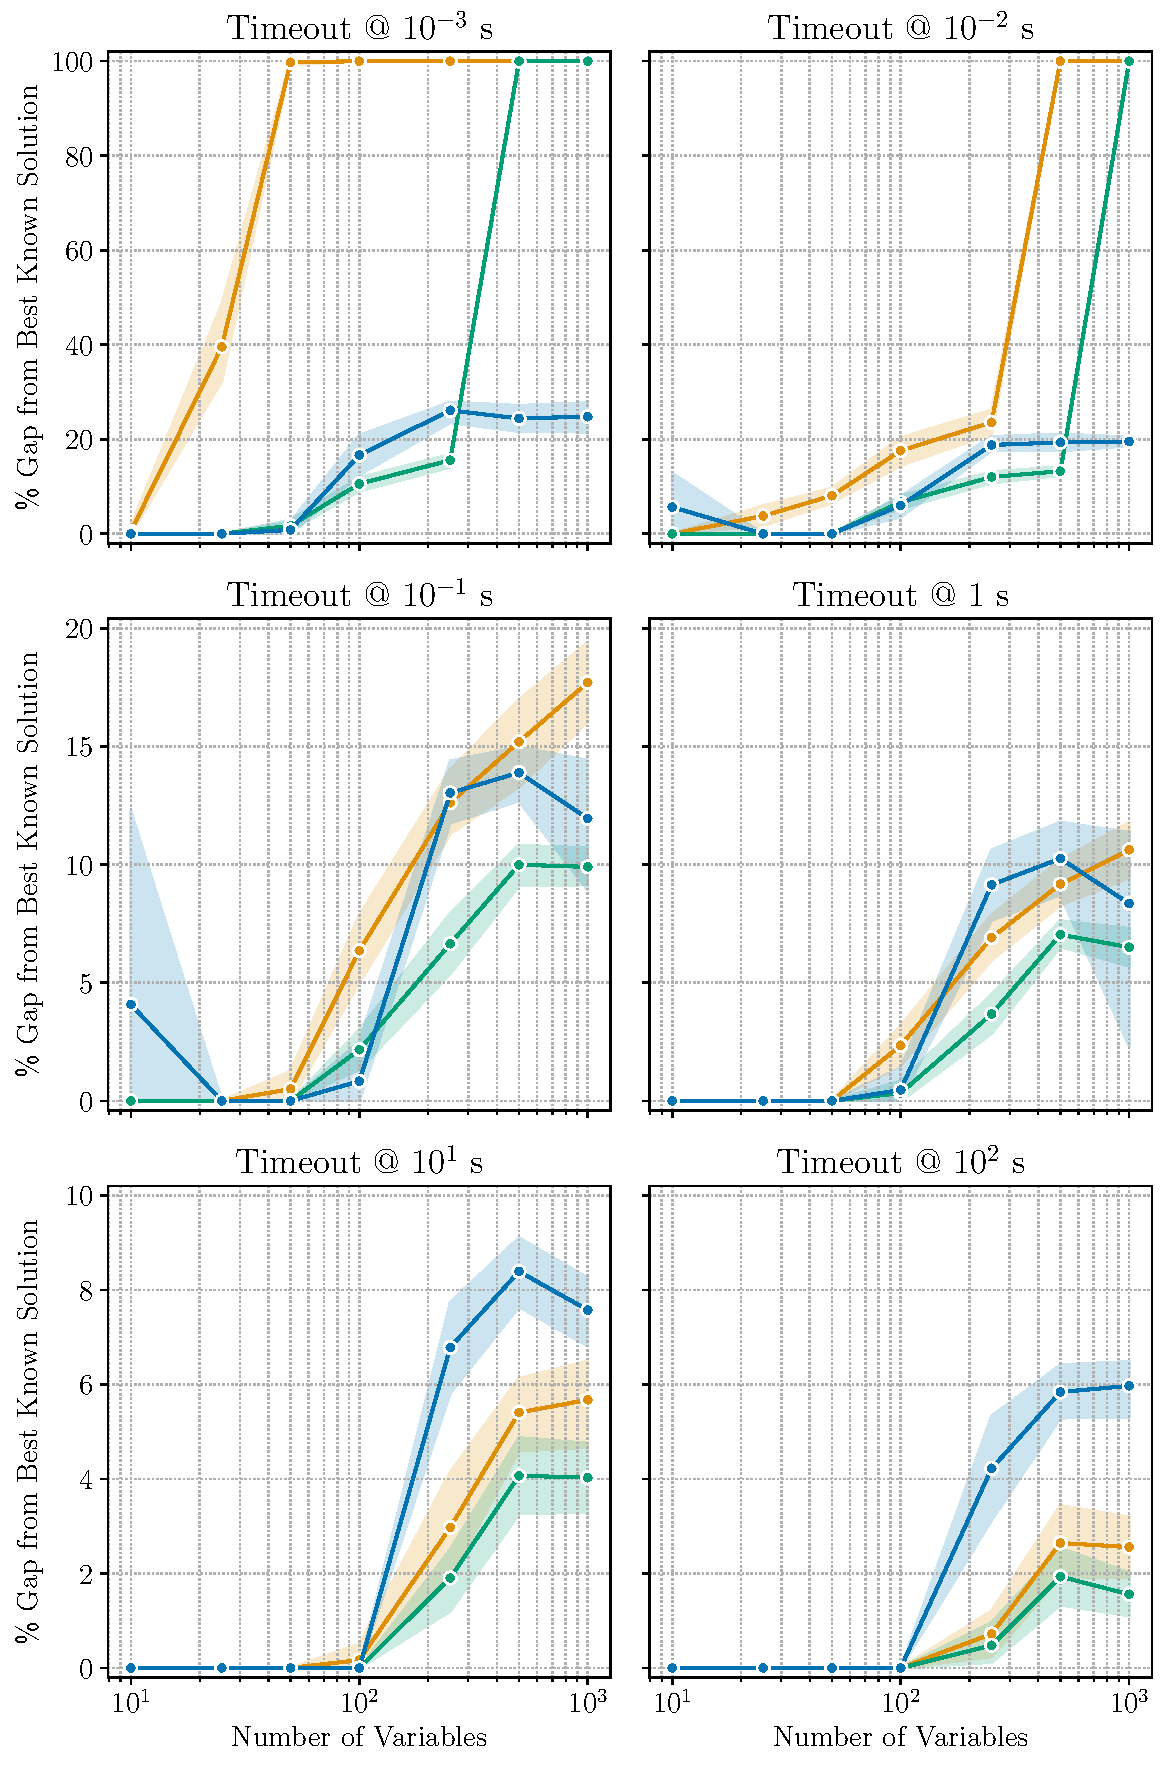
\includegraphics[width=\linewidth]{figures/mis_optimality_0.15.pdf}
    \vspace*{0.2cm}
    \end{subfigure}\\
    \begin{subfigure}{0.3\textwidth}
        
\includegraphics[width=\linewidth]{figures/legend.pdf}
    \end{subfigure}
    \caption{\secondrev{Percentage gap from the best known solution (BKS-Gap\%) for the QUBO workloads with QUBO matrices at $15\%$ density (lower is better). Results are shown for different timeouts of the QUBO solvers. Figure taken, with permission, from Pierro et al.~\cite{pierro2024solvingquboloihi2}.}}
    \label{fig:qubo_bksgap}
\end{figure}

\begin{figure}[t]
    \centering
        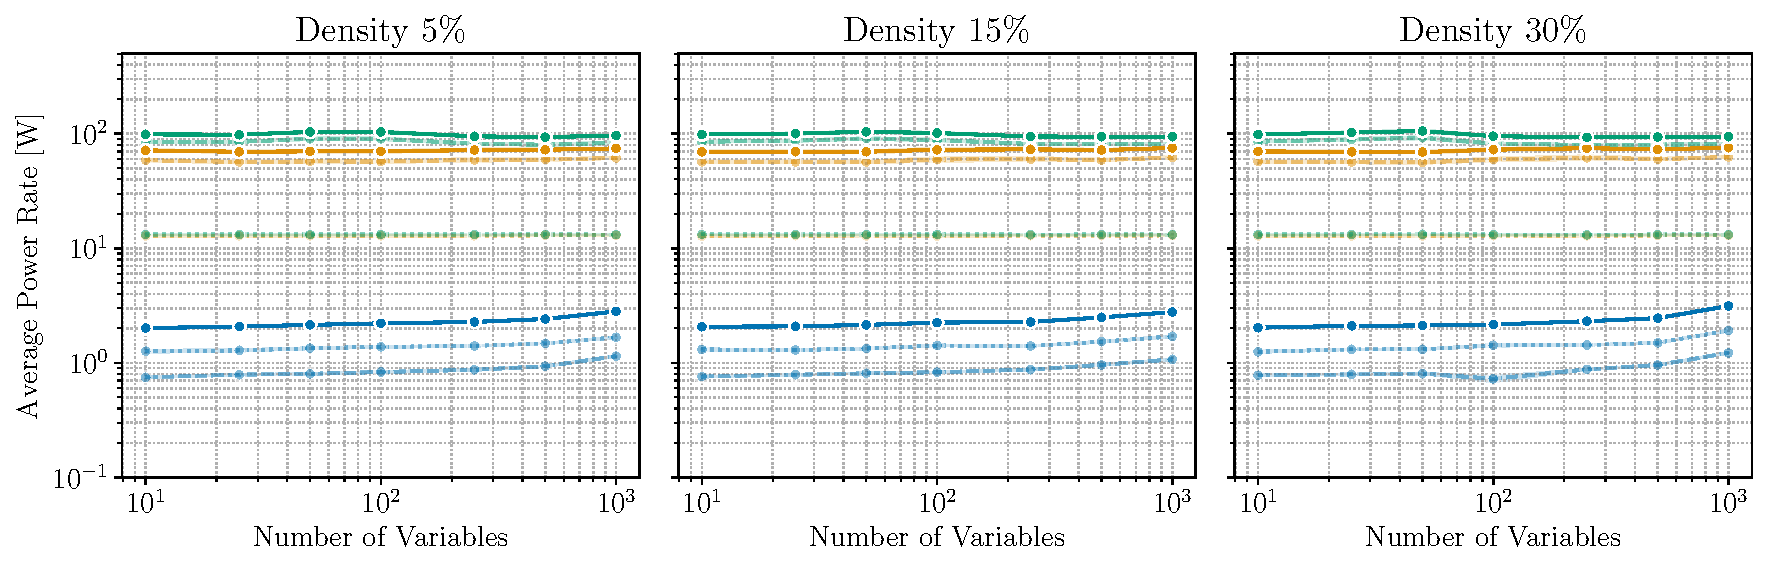
\includegraphics[width=\linewidth]{figures/mis_power.pdf}
    \vspace*{0.5cm}

\includegraphics[width=0.3\linewidth]{figures/legend.pdf}
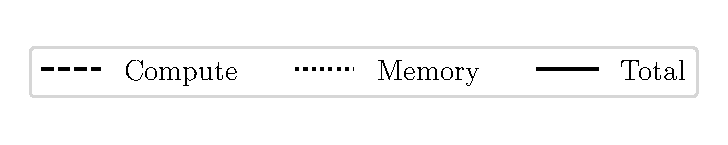
\includegraphics[width=0.35\linewidth]{figures/line_style_legend.pdf}
        \caption{\secondrev{Power consumption of the QUBO solvers running simulated annealing (SA) or TABU search on CPU, and the parallelized version of simulated annealing on Loihi 2. The CPU solvers require up to $37\times$ more power than the neuromorphic algorithm on Loihi 2. Since the QUBO workloads were run for a fixed timeout, differences in power consumption are equivalent to differences in energy consumption of the processors. Figure taken, with permission, from Pierro et al.~\cite{pierro2024solvingquboloihi2}.}}
        \label{fig:qubo_power}
\end{figure}

\secondrev{Three baselines are measured for the QUBO benchmark:
\begin{itemize}
    \item \textbf{Simulated Annealing (SA)} -- The simulated annealing solver uses Markov chain Monte Carlo (MCMC) sampling to probabilistically explore the search space. 
    \item \textbf{Tabu Search (TABU)} -- Tabu search solvers maintain and iterate a list of prohibited actions in order to prevent the search from remaining in local minima or revisiting states. Both the TABU and SA solver baselines use the D-Wave Samplers library~\cite{dwavesamplers} on an Intel Core i9-7920X desktop-class CPU, with power measured using Intel SoC Watch.
    \item \textbf{Loihi 2} -- The Loihi 2 neuromorphic system solver uses an SNN formulation of the simulated annealing algorithm which enables solving via neural dynamics, and parallelization via stochastic refractory periods. The baseline is implemented on one Loihi 2 chip on the 8-chip Kapoho Point board, and internal power instrumentation measures all compute and memory components of the chip.
\end{itemize}}

\secondrev{Figure~\ref{fig:qubo_bksgap} shows the optimality reached by the CPU- and Loihi 2-based solvers after different timeouts. For tight time constraints, at $10^{-2}$ seconds timeout or less, Loihi 2 finds feasible solutions to workloads $4\times$ larger than the CPU. But for timeout lasting $10$ seconds or longer, the CPU running TABU provides the lowest BKS-Gap, incentivizing algorithmic advances for neuromorphic optimization systems.}
\secondrev{Figure~\ref{fig:qubo_power} illustrates the power consumed during runtime. Across the workloads, the Loihi 2 solver requires $37.24\times$ less power compared to the best CPU solver.  
%All details on the solvers, benchmarking routine, and results have been provided by Pierro et al.~\cite{pierro2024solvingquboloihi2}.
}

\subsubsection*{Discussion and Future Work}
\secondrev{The initial baselines for the v1.0 system track compare correctness, timing, and efficiency of neuromorphic systems against conventional CPU systems in domains of both audio classification and optimization. Against mature, commercially-developed CPU systems, for both edge and server use cases, the neuromorphic systems show strong advantages in general efficiency, as well as further promises in terms of timing and correctness. 
%The benchmarks utilize collaboratively-defined task and methodology specifications, setting the groundwork for head-to-head neuromorphic system comparisons that will identify neuromorphic strengths and push towards standardization and development of better neuromorphic systems.
}

\secondrev{In future NeuroBench iterations, the system track benchmarks can be unified under common tooling, similar to the algorithm track. Software toolchains such as Lava~\cite{lava}, Fugu~\cite{aimone2019composing}, SPyNNaker~\cite{spynnaker}, and Samna~\cite{samna}, among others, have been developed to interface with specific hardware platforms. Many of the stacks are built with general paradigms to support extension to any backend, and the community is actively moving towards developing standards for deployment tools. The current v1.0 benchmark specifications allow for open algorithm and software design in order to demonstrate fully optimized performance for neuromorphic systems. As standards mature in the future, a core focus of the NeuroBench system track is to introduce a closed-algorithm benchmarking category that leverages the recently proposed NIR model description framework~\cite{NIR2024} as a general, cross-platform tool for benchmarking key workloads of interest across many different platforms.}